\section{Future Work}
\label{sec:concl.future}

This section touches on topics that were not covered extensively in this thesis or may be explained with results of this thesis.
It is divided into three logical parts.

First, the theory of the halved archetypal model was fully developed in the later part of this thesis.
It may be possible to explain the regularities of the bifurcations at the boundaries of ``type B'' parameter regions as they are described in \Cref{sec:arch.bif.sum}.
The regularities being that at the upper boundary of a ``type A'' parameter region, the border collision bifurcation is $\BCB_{d1, d_2}^{\underline{\A}^a\B^b\underline{\C}^a\D^b}$ while at the upper boundary of a ``type B'' parameter region, there are two border collision bifurcations $\BCB_{d_1}^{\underline{\A}^a\B^b\C^c\D^d}$ and $\BCB_{d_3}^{\A^c\B^d\underline{\C}^a\D^d}$.
Note that in the ``type A'' parameter boundary border collision bifurcation, two points of the branches $f_\A$ and $f_\C$ collide with the borders $d_1$ and $d_3$ respectively.
While in the ``type B'' border collision bifurcations this distributes onto both border collision bifurcations.
Here, the point of the branch $f_\A$ collides with the border $d_1$ for the cycle $\Cycle{\A^a\B^b\C^c\D^d}$ and the point of the branch $f_\C$ collides with $d_3$ for the cycle $\Cycle{\A^c\B^d\C^a\D^b}$.
The interesting part is that this distribution inverts for the lower boundary.
At the lower boundary, the point of the branch $f_\D$ collides with the border $d_3$ for the cycle $\Cycle{\A^a\B^b\C^c\D^d}$ and the point of the branch $f_\B$ collides with the border $d_1$ for the cycle $\Cycle{\A^c\B^d\C^a\D^b}$.
And for the right and left boundaries of the parameter regions this distribution of border collisions onto two bifurcations in the case of ``type B'' parameter regions is similar.

Second, \Cref{sec:arch.end} describes how the chains of parameter regions associated with the same period start falling apart for larger values of $\beta = c_L$.
This agrees with the behavior of the original model where the chains also start falling apart for larger values of $\chi_0$.
Nonetheless, this thesis proposes ways to obtain full chains with the archetypal model or a similar model.
These could be investigated in future work.

Third, there is another kind of bifurcation structure that the archetypal model can exhibit.
It is possible if the parameter $a_L$ is increased.
\Cref{fig:concl.fut.addincr} shows this bifurcation structure.
In this figure we can see \gls{pa} and \gls{pi} incrementing behavior close to each other.
On the left side there is \gls{pa} and on the right side there is \gls{pi}.
A similar bifurcation structure was observed in~\cite{AvrSchBan06}.
It would be interesting to investigate, how this bifurcation structure is affected by the symmetry in the archetypal model.
And if it is affected similarly to the \gls{pal} structures in this thesis, the algorithms developed here may be used to derive rules for this bifurcation structure as well.

\begin{figure}
	\centering
	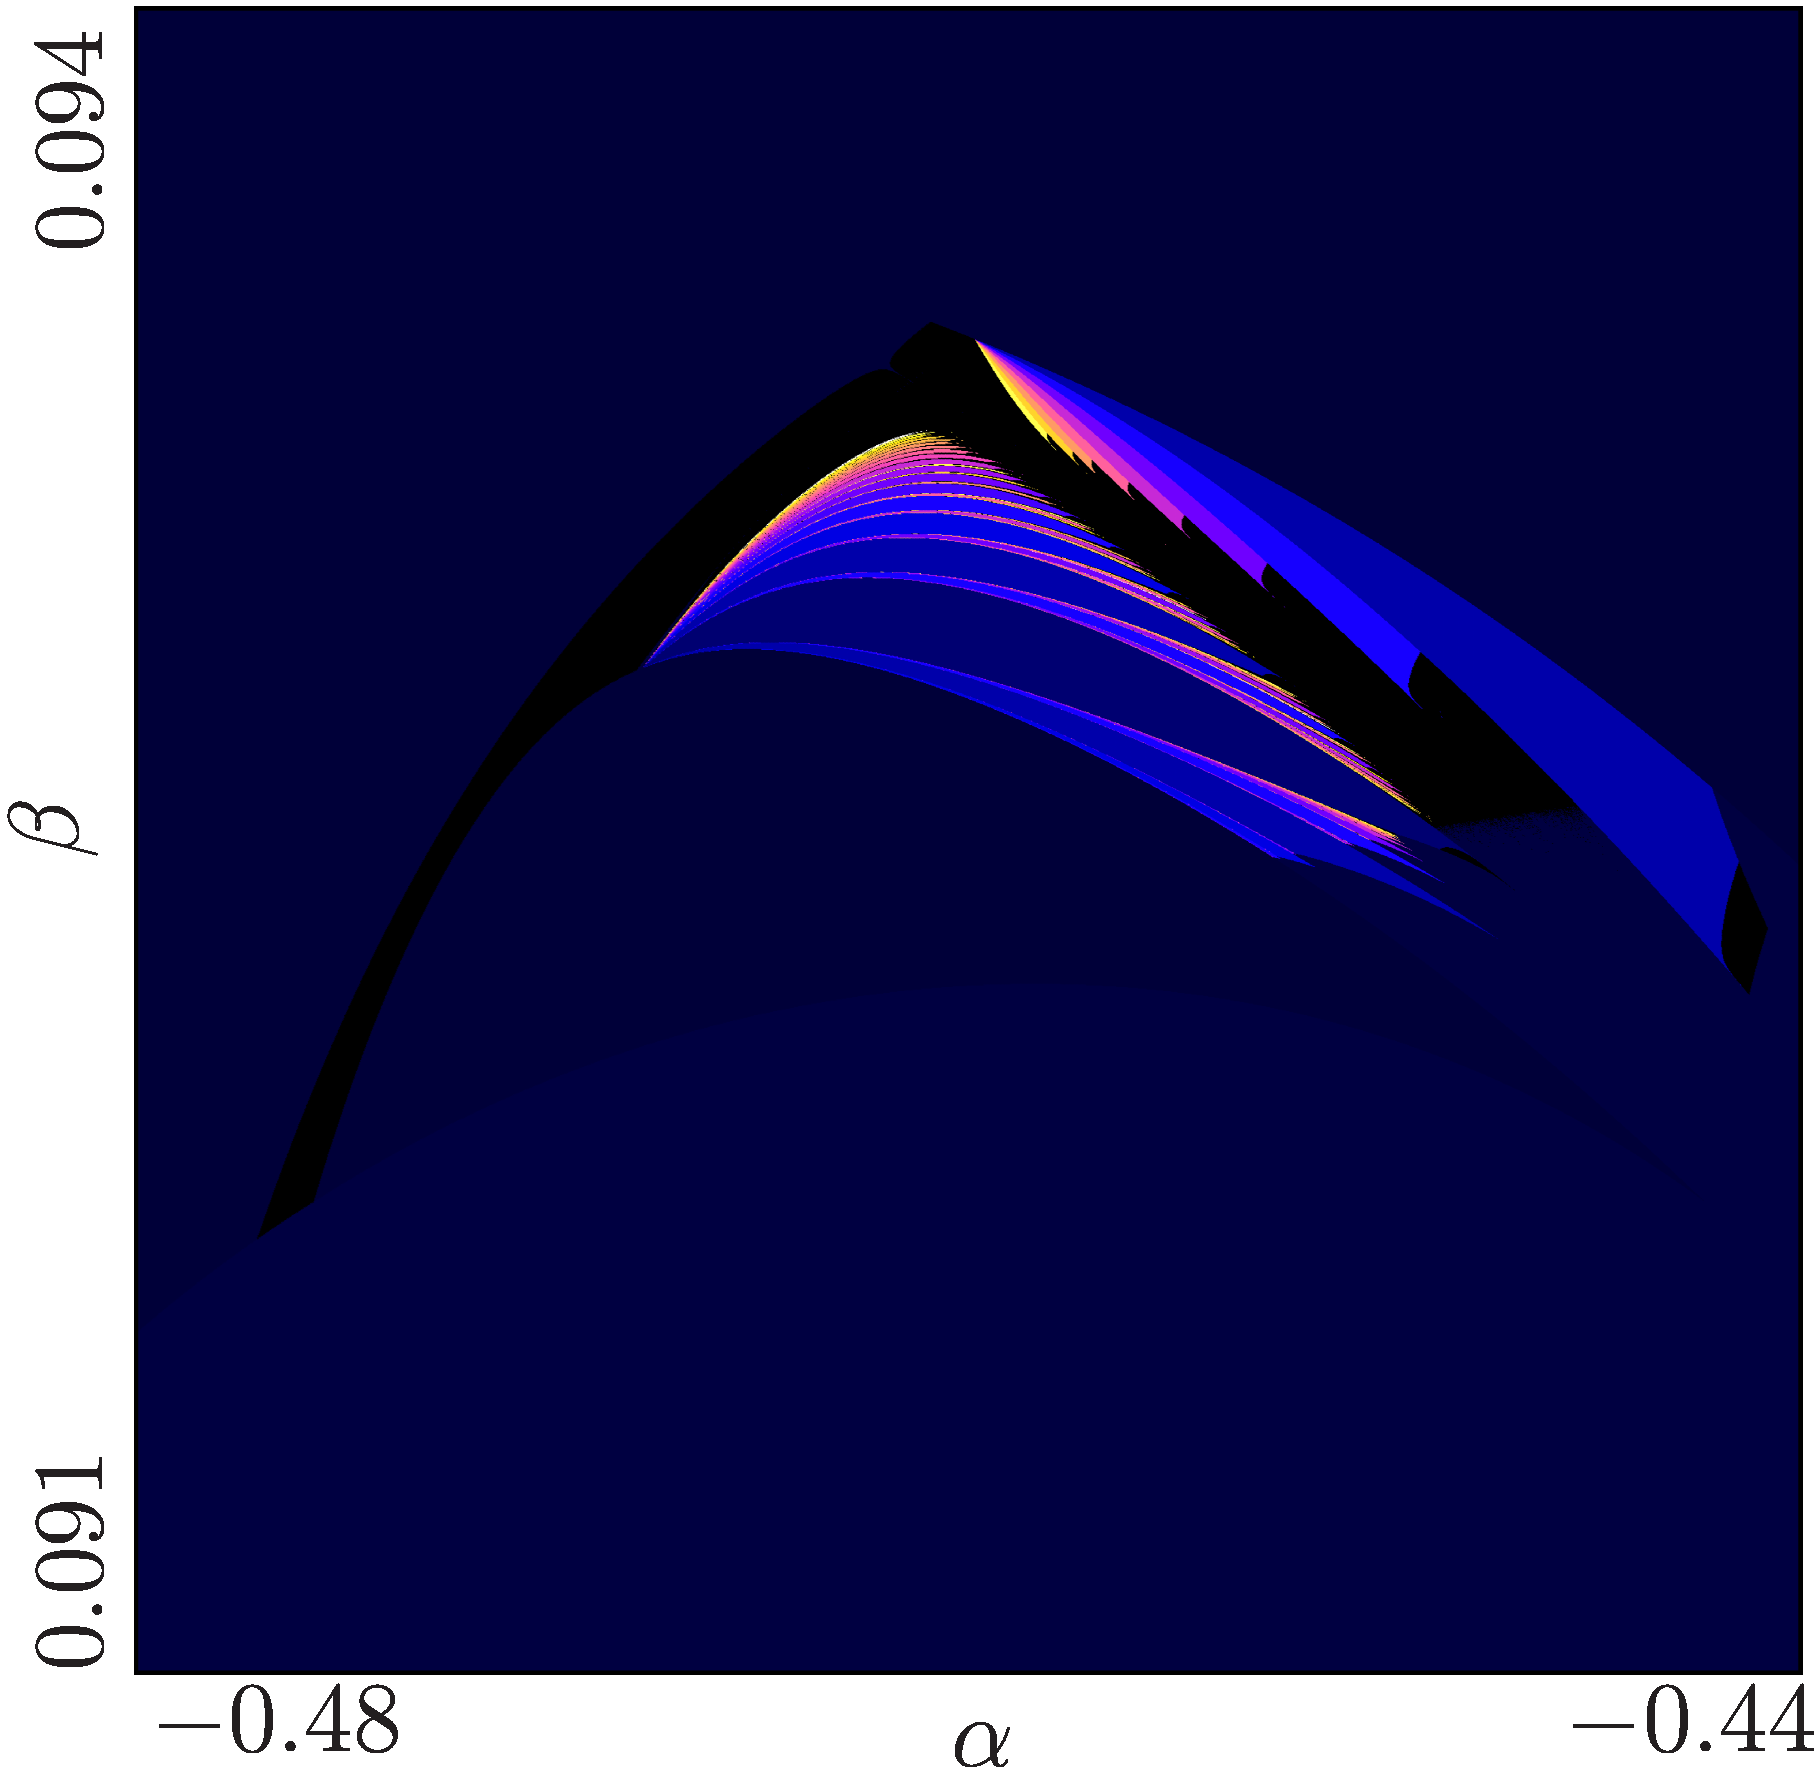
\includegraphics[width=.7 \textwidth]{../Figures/8/8.1/result.png}
	\caption[2D scan of the periods associated with parameter regions in the archetypal model with steep branches showing an interesting bifurcation structure]{
		2D scan of the periods associated with parameter regions in the archetypal model with steep branches showing an interesting bifurcation structure.
		The parameters $a_L = 8, b_L = -\frac{1}{2},$ and $g_R\left(\frac{1}{2}\right) = \frac{1}{2} + \frac{1}{40}$ are fixed.
		The parameters $\alpha = g_R\left(\frac{1}{4}\right)$ and $\beta = c_L$ are varied in the ranges $[-0.48, -0.44]$ and $[0.091, 0.094]$.
	}
	\label{fig:concl.fut.addincr}
\end{figure}
